\chapter{Эволюция одномерной вейбелевской турбулентности}\label{ch:ch1}
\section{Введение}\label{sec:ch1/sec1}

Среди неустойчивостей анизотропной плазмы апериодическая неустойчивость вейбелевского типа~\cite{Weibel1959,Zhou2022,Fried1959,Kalman1968,Morse1971,Kocharovsky2016,Lazar2006,Stockem2009,SchaeferRolffs2006} обладает одним из наибольших инкрементов и вместе с тем не сопровождается сильными резонансными нелинейными эффектами, поскольку ограничивается формированием квазимагнитостатических филаментов тока и не приводит к непосредственному возбуждению каких-либо волн. 
Но несмотря на то что в линейном приближении вейбелевская неустойчивость изучена достаточно подробно, особенно для бимаксвелловского распределения частиц~\cite{Weibel1959,Fried1959,Vagin2014}, существующая полностью аналитическая квазилинейная теория эволюции вейбелевской турбулентности разработана лишь в одномерной (1D2V) геометрии, причем для весьма ограниченной области параметров и без должного описания временной эволюции~\cite{Pokhotelov2011}. 
Вдобавок, открытым остается вопрос о применимости используемых в этой теории приближений, а следовательно, корректности полученных результатов.  
Полуаналитическое решение системы квазилинейных уравнений в 1D3V геометрии~\cite{Ruyer2015,StockemNovo2015} с опорой на эмпирические данные численного моделирования также применимо лишь для небольшой области параметров плазмы. 

В этой главе последовательно выведена оригинальная квазилинейная система уравнений и с ее помощью описана эволюция спектра возникающей турбулентности в простейшей постановке одномерной задачи на основе оригинального численного кода.
В развиваемом численном квазилинейном подходе функция распределения частиц и электрическое и магнитное поля представлены в виде сумм пространственных мод (гармоник), удовлетворяющих самосогласованным квазилинейным уравнениям, в которых все нелинейные явления обусловлены совместным действием мод на форму средней по пространству функции распределения частиц по скоростям. 
Последняя определяет текущие значения инкрементов (декрементов) и, возможно, действительных частот всех рассматриваемых мод, в остальном эволюционирующих независимо~\cite{Kuznetsov2023}. 
В результате, в отличие от метода частиц в ячейках, кардинально снижается уровень шумов и удается получать спектры вейбелевской турбулентности в гораздо более высоком качестве и в недоступных ранее областях параметров, правда, ценой потери некоторых слабых нелинейных эффектов при использовании сравнимых или даже б\'{о}льших вычислительных ресурсов.

Для определенности в конкретных расчетах ниже будем выбирать начальную функцию распределения частиц по скоростям бимаксвелловской, считая температуру частиц наибольшей вдоль оси $y$, называемой осью анизотропии. 
Для простоты будем предполагать плазму и все поля в ней однородными вдоль этой оси и оси $z$, т.е. решать систему уравнений Максвелла~-- Власова~\cite{Baumjohann2012} в одном (по координате $x$) измерении, а следовательно, полагать нулевыми проекции волновых векторов мод $\vec{k}$ на ось анизотропии: $k_y=0$ и на направление вдоль магнитного поля: $k_z=0$. 
При этом в каждой моде электрическое поле $\vec{E}$ направлено вдоль оси анизотропии, а магнитное $\vec{B}$ ортогонально ей и волновому вектору $\vec{k}$ (ТЕМ-моды). 

Главная цель представленной главы состоит в обосновании квазилинейного приближения и изучении в одномерном приближении нелинейных явлений квазилинейного типа, доминирующих в процессе развития вейбелевской турбулентности. 
Насколько нам известно, последовательный квазилинейный анализ ее эволюции до сих пор никем не проводился ни для какой анизотропии начальной функции распределения частиц по скоростям (ср., например,~\cite{Ruyer2015,Pokhotelov2011,Davidson1972}). 
Более того, другими авторами не проводилось даже достаточно длительное моделирование динамики спектра вейбелевских мод в простейшей постановке задачи об одномерной (1D2V) турбулентности, которой посвящена данная глава. 
Вместе с тем, некоторые выявленные особенности эволюции спектра и динамики отдельных мод аналогичны численно найденным ранее в других постановках задачи о вейбелевской турбулентности.

Последовательное обоснование и схема решения квазилинейных уравнений поясняется в разделе~\ref{sec:ch1/sec2} на примере одномерной задачи для дискретных мод с коллинеарными волновыми векторами, имеющими только компоненты $k_x$. 
Результаты численного исследования особенностей динамики соответствующей одномерной квазилинейной вейбелевской турбулентности и их сравнение с результатами имеющейся аналитической теории даны в разделе~\ref{sec:ch1/sec3} .


\section{Адиабатическая динамика мод и схема их связи в условиях слабого четырехволнового взаимодействия}\label{sec:ch1/sec2}

Для бесстолкновительной плазмы, в которой на рассматриваемых временах эволюции вейбелевской турбулентности можно пренебречь движением тяжелых ионов, самосогласованные уравнения  Максвелла~-- Власова для электрического $\vec{E}=(0, E_y, 0)$ и магнитного $\vec{B}=(0, 0,B_z)$ полей и функции распределения электронов $f(v_x , v_y , x, t)$ имеют вид~\cite{Vlasov1967,Kocharovsky2016}
\begin{align}
     \label{eq:maxw1} 
    \nabla \times \vec{B}=\dfrac{1}{c}\dfrac{\partial \vec{E}}{\partial t}+\dfrac{4\pi}{c}\vec{j}, \\
    %
    \label{eq:maxw2}
    \nabla \times \vec{E}=-\dfrac{1}{c}\dfrac{\partial \vec{B}}{\partial t}, \\
    %
    \dfrac{\partial f}{\partial t}+\vec{v}\dfrac{\partial f}{\partial \vec{r}}+\dfrac{e}{\me} \left(\vec{E}+\dfrac{1}{c}\left[\vec{v},\vec{B}\right]\right) \dfrac{\partial f}{\partial \vec{v}}=0,
    \label{eq:Vlasov}
\end{align}
где $c$~--- скорость света в вакууме, $e$ и $\me$~--- заряд и масса электрона, $\vec{j}=e\iint^{+\infty}_{-\infty}\vec{v}f(v_x , v_y , x, t) dv_x dv_y$~--- плотность тока, $N=\iint^{+\infty}_{-\infty}f(v_x , v_y , x, t)dv_xdv_y$~--- концентрация электронов. 
Здесь и ниже в главах~\ref{ch:ch1} и \ref{ch:ch2} речь идет о так называемых ТЕМ-возмущениях, в которых взаимно ортогональны друг к другу волновой вектор и магнитное и электрическое поля, причем последнее параллельно оси анизотропии плазмы. 
В главе \ref{ch:ch2} речь пойдет о двумерной задаче, в которой радиус-вектор является двухкомпонентным, $\vec{r}=(x , 0 , z)$, а вектор скорости~--- трехкомпонентным,  $\vec{v}=(v_x , v_y ,v_z)$ (в одномерной задаче отсутствуют зависимости от координаты $z$ и скорости $v_z$, но сохраняются зависимости от двух других компонент $v_x$, $v_y$). 

Положим, что в начальный момент времени нормированная функция распределения по скоростям $c^3f/N$ имеет бимаксвелловский вид:
\begin{equation}
\label{bimax}
\Psi({\beta})=\dfrac{1}{\pi^{3/2}\beta_{\perp0}^2 \beta_{\|0} } \exp\left(-\dfrac{\beta_x^2+\beta_z^2}{\beta_{\perp0}^2}-\dfrac{\beta_y^2}{\beta_{\|0}^2}\right).
\end{equation}
Здесь $\beta_{x,y,z}={v_{x,y,z}}/{c}$, т.\,е. ${\beta}=\vec{v}/{c}$, и в дальнейшем используется параметр анизотропии $A_0={\beta^2_{\|0}}/{\beta^2_{\perp0}}-1$, определяемый отношением большей тепловой скорости к меньшей.


Квазилинейный подход к описанию ТЕМ-вейбелевской неустойчивости основан на разложении по пространственным модам (гармоникам) решения уравнений  Максвелла~-- Власова~\cite{Baumjohann2012} с шумоподобным начальным возмущением магнитного поля, обладающим примерно равномерным спектром в области неустойчивых волновых чисел мод.
Особенно эффективным подобное разложение является тогда, когда ключевую роль играет интегральное нелинейное взаимодействие мод посредством их совместного изменения средней по пространству функции распределения частиц по скоростям. 
Для вейбелевской турбулентности это оправдано ввиду слабой нелинейности кинетического уравнения Власова в рассматриваемых условиях отсутствия квазимонохроматических электромагнитных волн и их резонансного взаимодействия ~\cite{Weibel1959,Davidson1972,Silva2020}.


В частности, как показали тестовые расчеты, для любой отдельной гармоники магнитного (и соответствующего электрического) поля $B_1(t,x)= \mathrm{Re} \left[ B_1(t)\exp(-\mathrm{i}kx) \right]$ с волновым вектором $\vec{k}$, для определенности направленным вдоль орта $\vec{x_0}$, можно не учитывать кратные гармоники $\ell k$ с целым $\ell > 1$ и необходимо учесть только три гармоники поправок к функции распределения, $\delta f_\ell(t, x)=\mathrm{Re} \left[ f_\ell(t)\exp(-\mathrm{i}\ell kx) \right]$, со значениями $\ell =$ 0, 1, 2. 
При этом возбуждение чётной гармоники $\ell=$ 2 магнитного поля фактически невозможно благодаря ограничениям симметрии в одномерной задаче. 
Здесь и ниже $\vec{x}_0$, $\vec{y}_0$, $\vec{z}_0$~--- единичные орты декартовой системы координат. 

Наличие большого числа однотипных не сфазированных мод, достаточно плотно заполняющих значимую область волновых векторов, гарантирует гладкость формы и плавность изменения функции распределения, исключая артефакты когерентной интерференции и отрицательные значения функции распределения электронов всюду, кроме, возможно, несущественной, содержащей крайне мало частиц, области их скоростей, очень больших по сравнению с тепловыми скоростями. 
При этом по существу реализуется адиабатическая динамика каждой моды, непрерывно подстраивающейся к изменяющейся функции распределения частиц. 
Корректность такого рода теории возмущений, а фактически~--- соблюдение иерархии малости амплитуд последующих гармоник по сравнению с предыдущими (как гармоник функции распределения, $|\delta f_ \ell|\gg |\delta f_{\ell+1}|$, так и аналогичных гармоник магнитного или электрического полей) проверены в случаях задания одной или двух производящих мод. 

Так, в случае единственной производящей моды нелинейно связываются все кратные гармоники функции распределения $\ell k$ с $\ell =$ 0, 1, 2, 3,~... и нечетные гармоники ТЕМ-поля $\ell k$ с $\ell =$ 1, 3,~... (в силу отсутствия токов на четных гармониках из-за свойств четности функции распределения), но учет высших гармоник, начиная с $\ell =$ 3, почти не изменяет результат.  
Удостовериться в этом позволяет следующая система связанных уравнений для кратных (комплексных) гармоник-возмущений функции распределения, отвечающая теории возмущений до $\ell = 4$:

\begin{align}
\label{eq:furre5}
\vec{B} = \mathrm{Re} \left[ B_1(t) \exp(-\mathrm{i}kx)+B_3(t)\exp(-3\mathrm{i}kx)\right] \vec{z_0} ,\\
\label{eq:f0.1}
\dfrac{\partial f_0}{\partial t}+\hat \phi(\Omega_1,f_1^*)+\hat \phi^*(\Omega_1^*,f_1)+\hat \phi(\Omega_3,f_3^*)+\hat \phi^*(\Omega_3^*,f_3)=0,\\
\label{eq:f1.1}
\dfrac{\partial f_1}{\partial t}+\mathrm{i}kv_xf_1+2\hat \phi(\Omega_1,f_0)+\hat \phi^*(\Omega_1^*,f_2)+\hat \phi(\Omega_3,f_2^*)=0,\\
\label{eq:f2.1}
\dfrac{\partial f_2}{\partial t}+2\mathrm{i}kv_xf_2+\hat \phi(\Omega_1,f_1)+\hat \phi^*(\Omega_1^*,f_3)+\hat \phi(\Omega_3,f_1^*)=0,\\
\label{eq:f3.1}
\dfrac{\partial f_3}{\partial t}+3\mathrm{i}kv_xf_3+2\hat \phi(\Omega_3,f_0)+\hat \phi^*(\Omega_1^*,f_4)+\hat \phi(\Omega_1,f_2)=0,\\
\label{eq:f4.1}
\dfrac{\partial f_4}{\partial t}+4\mathrm{i}kv_xf_4+\hat \phi(\Omega_1,f_3)+\hat \phi(\Omega_3,f_1)=0,
\end{align}
где опущены очевидные осцилляторные уравнения для первой и третьей гармоник магнитного поля (\ref{eq:furre5}), получающиеся из уравнений (\ref{eq:maxw1}), (\ref{eq:maxw2}) и в силу их линейности включающие только соответствующие первую и третью гармоники функции распределения. 
Для сокращения записи здесь введён оператор
\begin{align}
\label{eq:oper.1}
    \hat{\phi}(\Omega_{n},f(\vec{v}))  =  \frac{\mathrm{i}}{2nk}\cdot\frac{\partial \Omega_{n}}{\partial t}\frac{\partial f(\vec{v})}{\partial v_y} -\frac{1}{2}\Omega_{n} \left(v_x\frac{\partial f(\vec{v})}{\partial v_y}-v_y\frac{\partial f(\vec{v})}{\partial v_x}\right)
\end{align}
и комплексная гирочастота $\Omega_n={e B_n}/{(\me c)}$.
Схема данной системы представлена на рис.~\ref{fig:1m2pribl_1}.
Она обаладает следующими свойствами:
\begin{enumerate}
\item Нелинейные слагаемые в нечетных гармониках ФР пропорциональны $\hat \phi(\Omega_1,\hat \phi(\Omega_1,f_1))$, а также $\hat \phi(\Omega_1,\hat \phi(\Omega_3,f_1))$ и $\hat \phi(\Omega_1,\hat \phi(\Omega_1,f_3))$. 
Нечетные гармоники магнитного поля взаимосвязаны через четные гармоники ФР.
\item Нелинейные слагаемые, определяющие насыщение экспоненциального роста первой гармоники, включают возмущения функции распределения на второй и нулевой гармонике. 
\item Отсутствует ненулевое стационарное решение  для нулевой гармоники $f_0$.
\end{enumerate}

\begin{figure}[h]
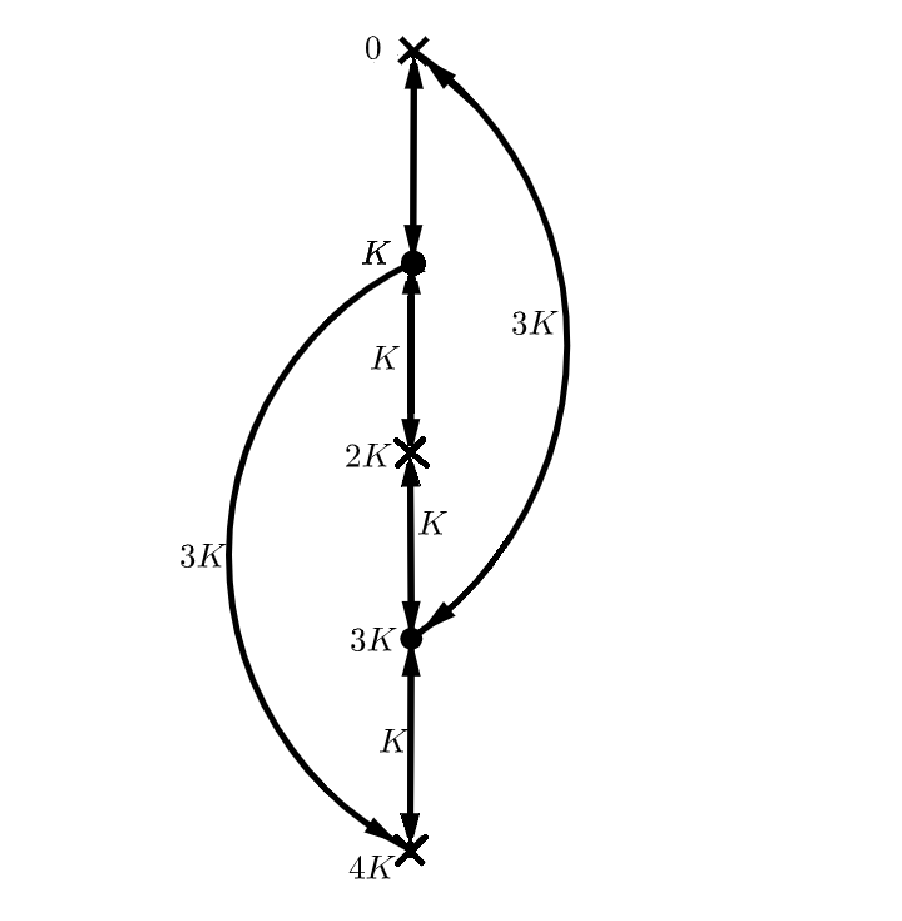
\includegraphics[width=0.4\linewidth]{part1/fig1.eps}
\centering
\caption{Схема связи четырех гармоник функции распределения частиц в самосогласованной системе уравнений (\ref{eq:furre5})--(\ref{eq:f4.1}) для одной производящей моды. 
Узел на схеме отвечает уравнению на соответствующую гармонику. Если поле некоторой гармоники тождественно равно нулю, то соответствующий узел изображен в виде крестика, а если нет~--- в виде точки. 
Входящая в узел стрелка отвечает слагаемому в уравнении для гармоники, соответствующей этому узлу. 
В таком слагаемом присутствует гармоника поля, соответствующая гармонике, указанной на стрелке, и гармоника функции распределения частиц, указанная на узле, из которого стрелка исходит.} 
\label{fig:1m2pribl_1}
\end{figure}

В том числе и в наиболее опасном случае высокой начальной анизотропии, при которой величина линейного инкремента наиболее неустойчивой вейбелевской моды $\gamma_{max}$ не слишком мала и сопоставима с произведением волнового числа  $K_{opt}$, для которого он достигается, на начальную поперечную тепловую скорость $\beta_{\perp0}$, проверено, что в численное решение полученной системы уравнений для параметра анизотропии $A$ и основной гармоники (моды) магнитного поля $B_1(t)$, непосредственно создаваемой первой гармоникой функции распределения $f_1(t)$, практически не отличается от численного решения значительно упрощенной системы, в которой эволюция данной гармоники $B_1(t)$ (и $f_1(t)$) определяется лишь согласованной динамикой нулевой и второй гармоник функции распределения $f_0,_2(t)$, но не третьей (и высшими) гармониками магнитного поля и функции распределения (рис.~\ref{fig:comparison1and2pribl}).
Этот результат реализуется вследствие слабости нелинейной генерации утроенной и последующих кратных мод $B_3(t)\ll B_1(t)$ (рис.~\ref{fig:evol_2pribl}).  Ниже будет показано, что нарушение именно этого, по существу иерархического условия условия слабости нелинейной генерации кратных мод, например, в присутстие достаточно сильного постоянного однородного магнитного поля, приводит к неприменимости развиваемого квазилинейного подхода.  

\begin{figure}[h]
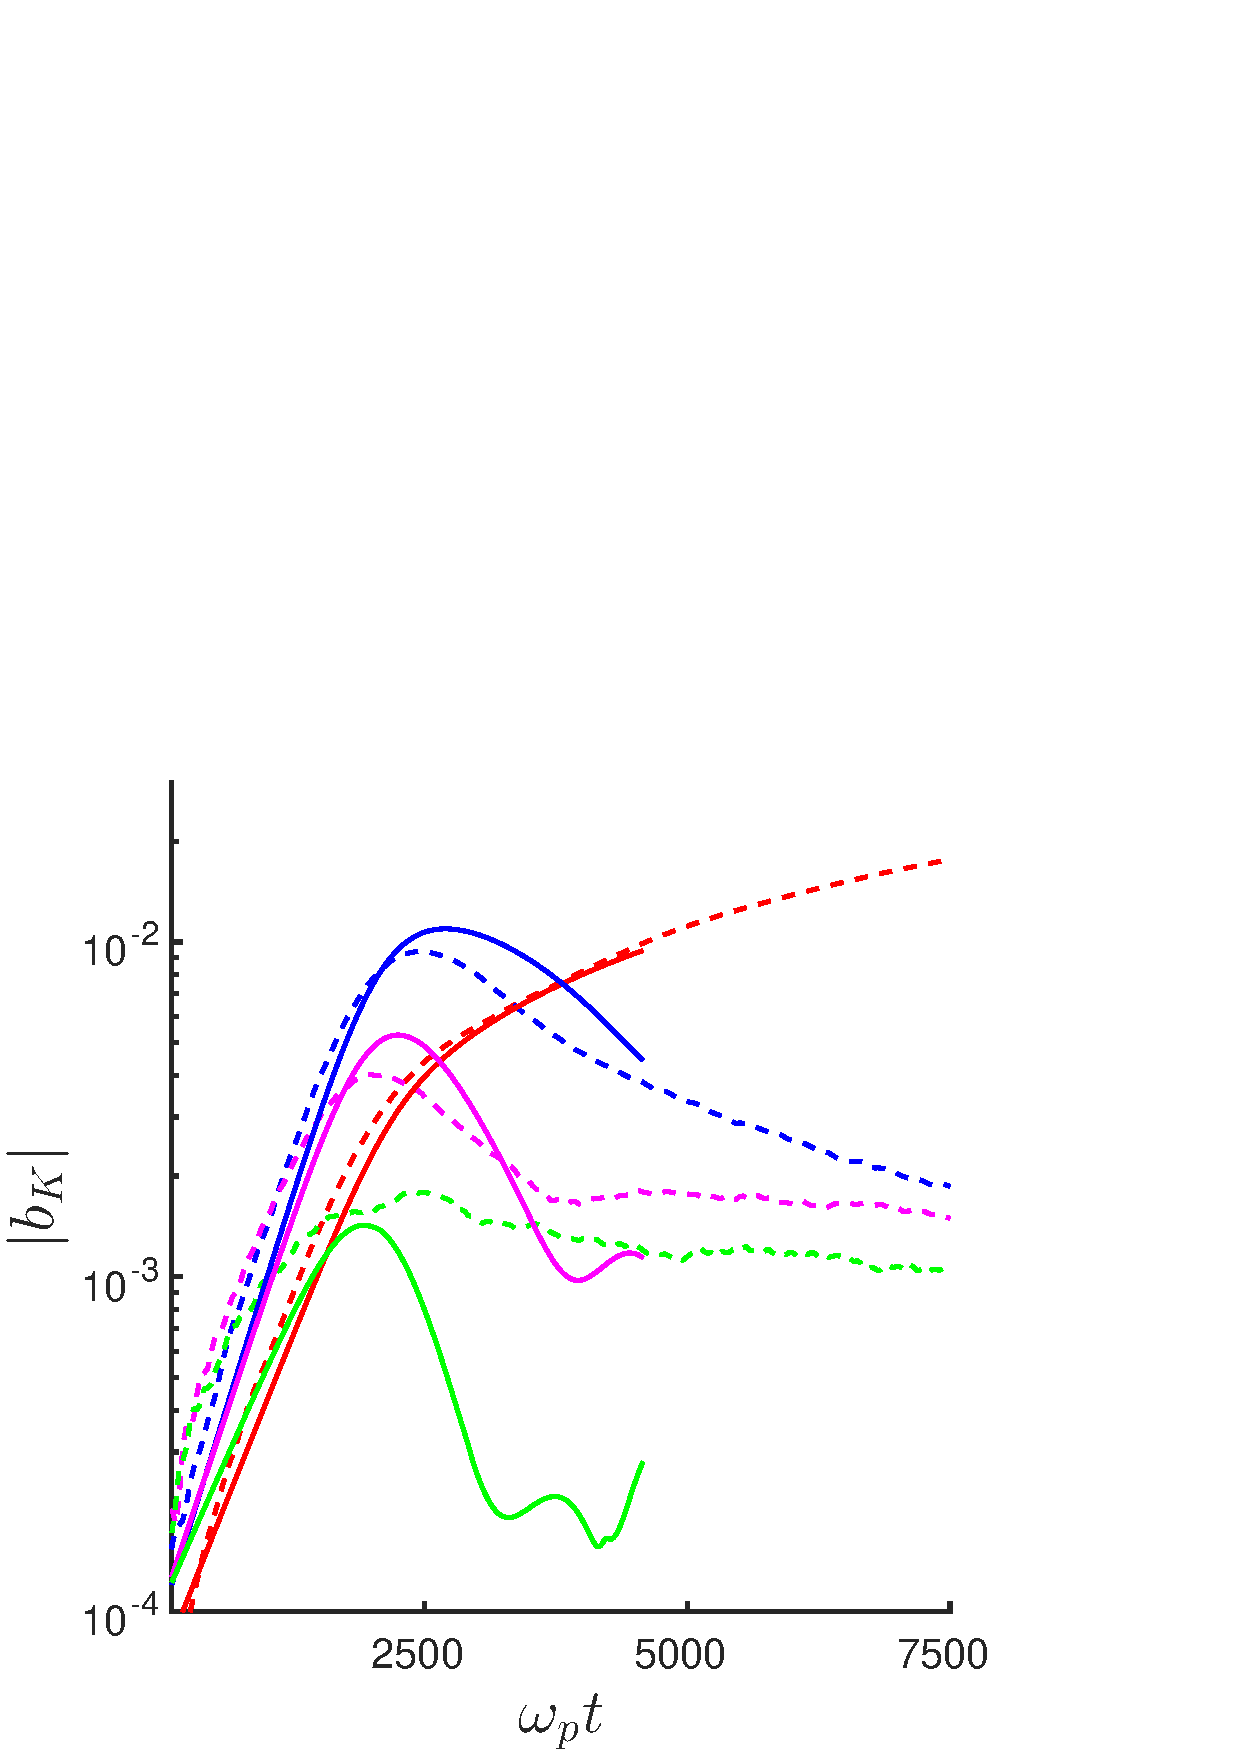
\includegraphics[width=0.6\linewidth]{part1/fig14.png}
\centering
\caption{Эволюция основной гармоники магнитного поля и показателя анизотропии с учетом утроенной и учетверенной гармоник (пунктир) и без них (сплошная) при $A=10$, $\beta_\perp=0.1$} 
\label{fig:comparison1and2pribl}
\end{figure}

\begin{figure}[h]
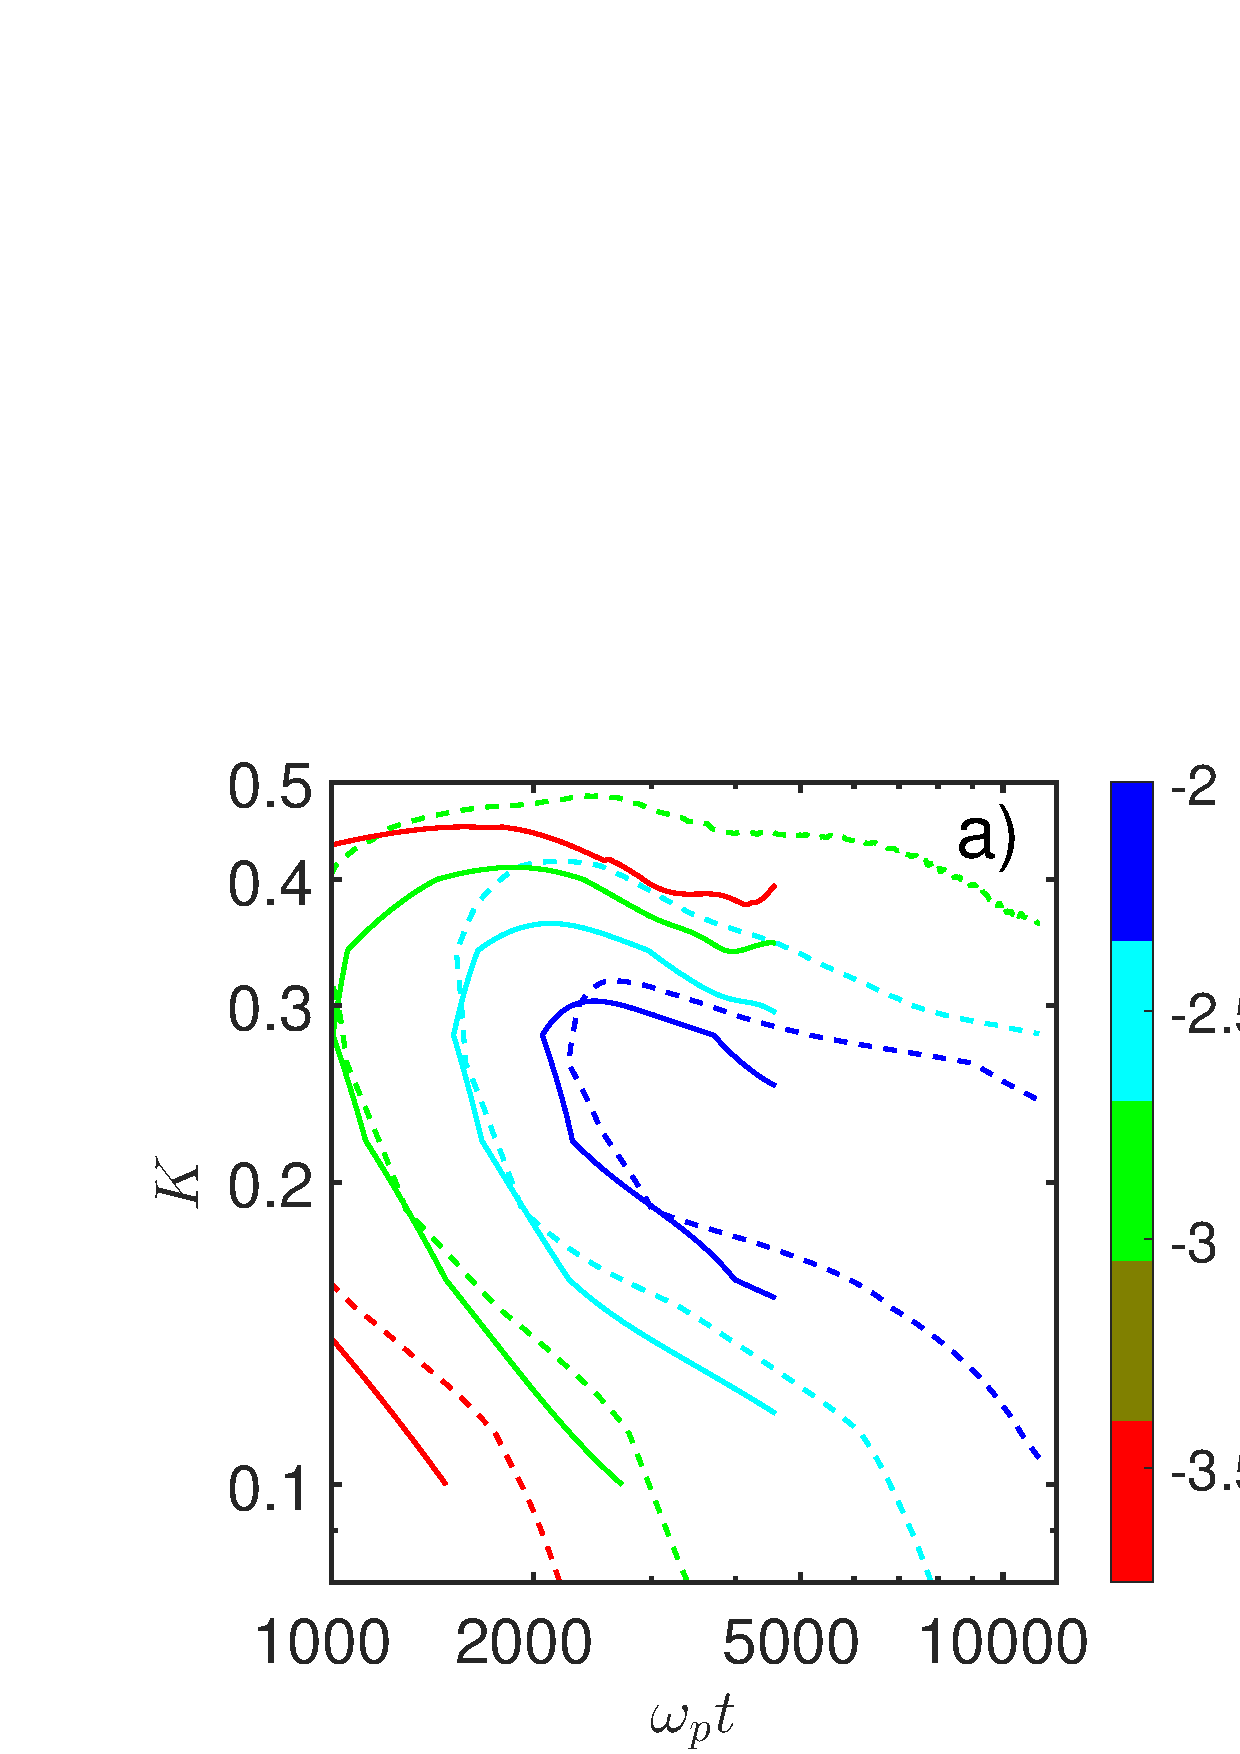
\includegraphics[width=0.4\linewidth]{part1/fig13.png}
\centering
\caption{Эволюция основной и утроенной гармоник в самосогласованной системе уравнений (\ref{eq:furre5})--(\ref{eq:f4.1}) для разных волновых чисел при $A=10$, $\beta_\perp=0.1$} 
\label{fig:evol_2pribl}
\end{figure}

В общем случае многомодовой динамики вейбелевской неустойчивости неизбежно возникают перекрестные гармоники вида $k_i\pm k_j$, $2k_i\pm k_j$ и т.д. 
Схема взаимосвязи подобных перекрестных гармоник в случае наличия двух производящих вейбелевских мод дана на рис.~\ref{fig:2m2pribl}. 

Подобно иллюстрации корректности пренебрежения кратными гармониками высокого порядка в одномодовом режиме, показана слабость влияния генерации перекрестных гармоник в случае начального задания только двух сильных мод. 
С этой целью вновь в наиболее опасном случае высокой начальной анизотропии для различных пар мод проведено сравнение численных решений более общей системы, представленной на рис.~\ref{fig:2m2pribl} и содержащей гармоники не выше второго порядка, включая суммарные и разностные, с численными решениями в квазилинейном подходе, в котором взаимодействие мод с различными не кратными волновыи числами осуществляется исключительно путем их совместной деформаци однородной компоненты распределения частиц. 
Наблюдаемые отличия в динамике отдельных мод крайне локализованы во времени, отличия в эволюции интегральных величин, таких как среднеквадратичное магнитное поле и текущая анизотропия, ничтожны и не превышают 1\% (рис.~\ref{fig:two_modes}).

\begin{figure}[h]
\centering
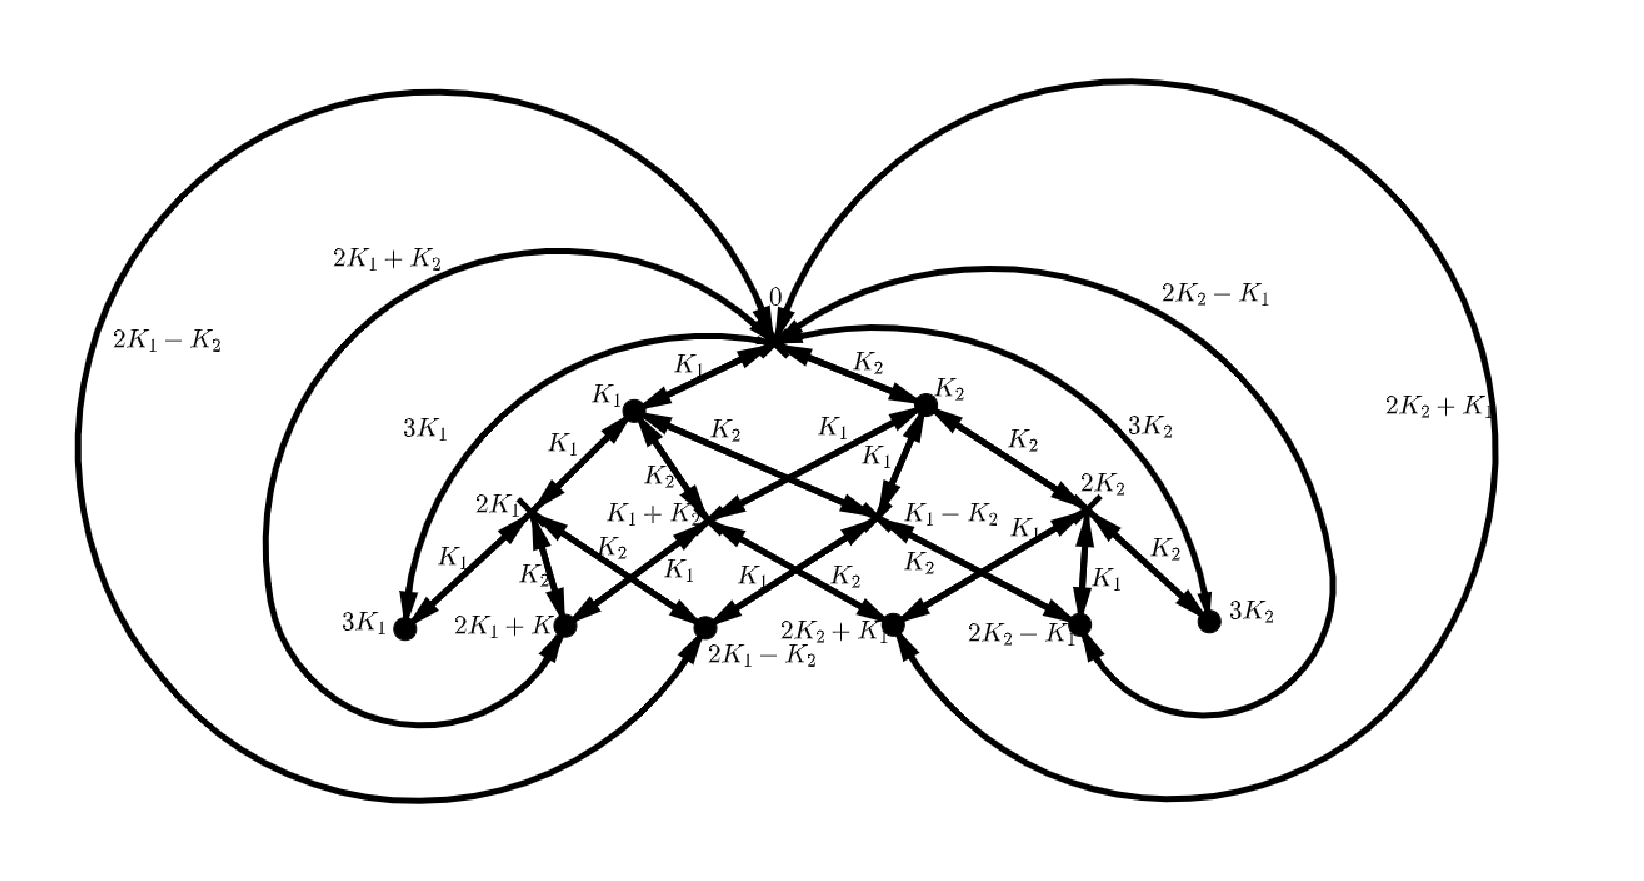
\includegraphics[width=1\linewidth]{part1/fig3.eps}
\caption{Схема связи гармоник функции распределения в самосогласованной системе уравнений для двух производящих мод. Обозначения те же, что на рис.~\ref{fig:1m2pribl_1}.}
\label{fig:2m2pribl}
\end{figure}

\begin{figure}[h]
\includegraphics[width=0.45\linewidth]{part1/evol2mode_Ka08Kg1_srav.eps}
\centering
\caption{Эволюция амплитуды магнитного поля двух взаимосвязанных мод с волновыми числами $k_1=0.8$ (красный цвет) и $k_2=1$ (синий цвет) в случае учета перекрестных гармоники вида $k_i\pm k_j$, $2k_i\pm k_j$ (сплошная) и в случае их отсутствия (пунктир). Черным цветом показана эволюция средневадратичного магнитного поля.}
\label{fig:two_modes}
\end{figure}

В дополнение к сказанному, проведена прямая провека корректности квазилинейного подхода путем сравнения решения упрощенной системы уравнений (\ref{eq:furre5})--(\ref{eq:f4.1}), из которой исключены учетверенная и утроенная гармониа, с полностью нелинейным решением исходных уравнений (\ref{eq:maxw1})--(\ref{eq:Vlasov}) кодом EPOCH при начальном возбуждении одной сильной моды существенно выше уровня шумов. 
В результате получено, что описанные решения совпадают с точностью до нескольких процентов~(рис.~\ref{fig:srav_PIC}), а значит, существует значимый промежуток нелинейной эволюции вейбелевской турбулентности, в течение которого квазилинейное приближения является достаточным для ее описания.

\begin{figure}[h]
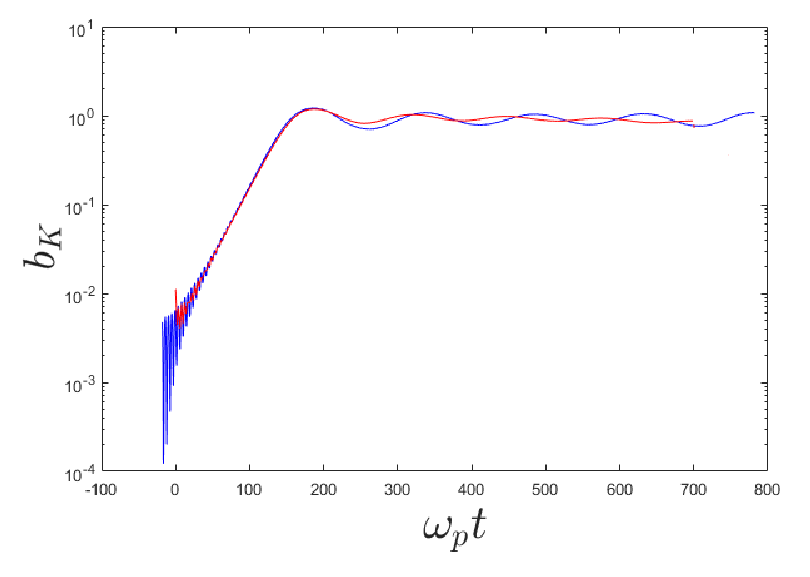
\includegraphics[width=0.4\linewidth]{part1/fig2.eps}
\centering
\caption{Эволюция одной моды: сравнение хода амплитуды основной гармоники магнитного поля в квазилинейном расчете по уравнениям (\ref{eq:f0.1})--(\ref{eq:f4.1}) (синий цвет) и в расчете методом частиц в ячейках с помощью кода EPOCH по уравнениям (\ref{eq:maxw1})--(\ref{eq:Vlasov}) (красный цвет) при $A_0=10$, $K=1.2$.}
\label{fig:srav_PIC}
\end{figure}


Таким образом, в отсутствие учета кратных гармоник вида $nk_i$, гдe $n\gg3$ и перекрестных гармоник вида $k_i\pm k_j$, $2k_i\pm k_j$ имеем следующую квазилинейную систему уравнений для одномерной вейбелевской турбулентности (рис. \ref{fig:multimode}) с большим числом $m$ коллинеарных мод $\{ k_1,\, k_2,...,\,k_{m} \}$, волновые векторы которых направлены поперек оси анизотропии, часто расположены и перекрывают всю существенную область неустойчивости: 
\begin{align}
\label{eq:f0.3}
\dfrac{\partial \psi_0}{\partial \tau}+\sum\limits^{m}_{n=1}\bigg(\hat \Phi(b_{K_n},\psi_{K_n}^*)+\hat \Phi^*(b_{K_n}^*,\psi_{K_n})\bigg)=0, \\
\label{eq:f1.3}
\dfrac{\partial \psi_{K_n}}{\partial \tau}+\mathrm{i}K_n\beta_x\psi_{K_n}+2\hat \Phi(b_{K_n},\psi_0)+\hat \Phi^*(b_{K_n}^*,\psi_{2K_n})=0, \\
\label{eq:f2.3}
\dfrac{\partial \psi_{2K_n}}{\partial \tau}+2\mathrm{i}K_n\beta_x\psi_{2K_n}+\hat \Phi(b_{K_n},\psi_{K_n})=0,\\
\label{eq:max_eq}
\ddot b_{K_n}+K_n^2b_{K_n}=\dfrac{\mathrm{i}K_n}{\beta_{||0}}\iint\limits^{\infty}_{-\infty}\beta_y\psi_{K_n}(\tau,\beta_x,\beta_y) d\beta_x d\beta_y.
\end{align}

Согласно ей, магнитное поле имеет вид суммы мод по целочисленному индексу $n$:
$B(t,x)= \mathrm{Re} \, \sum^{m}_{n=1}B_{k_{\vec{n}}}(t)\exp(- ik_{n}x)$.
Аналогичный вид имеет каждая из двух кратных гармоник-возмущений функции распределения частиц по скоростям, т.\,е. компонент $\delta f_1(t,x)$ и $\delta f_2(t,x)$, разложенных на комплексные гармоники ${f_1}_{k_{\vec{n}}}(t)$ и ${f_2}_{k_{\vec{n}}}(t)$ соответственно; нулевая (действительная) гармоника $f_0(t)=\delta f_0(t)$ зависит только от вектора скорости и дает поправку к функции распределения, усредненную по оси $x$. Здесь и ниже используются время и волновое число, нормированные на плазменные частоту и масштаб,
\begin{align}
\label{eq19plus2}
    \tau=\wpl t, \
    K=\dfrac{kc}{\wpl}; \ 
    \wpl^2=\dfrac{4\pi Ne^2}{\me}.
\end{align}

Комплексные амплитуды мод (гармоник) магнитного поля и функции распределения тоже нормированы:

\begin{align}
\label{eq19plus1}
    b_{K_{n}}=\dfrac{B_{K_{n}}}{\sqrt{8\pi N T_{\|0}}},\
    T_{\|0}=\dfrac{m_ec^2\beta_{\|0}^2}{2},\  \psi_{\ell\cdot K_{n}}=\dfrac{c^2f_{\ell\cdot K_{n}}}{N},
    \ \ell=0,\,1,\,2.  
\end{align}
Для многомодовой задачи введен оператор 
\begin{align}
\label{eq:oper.2}\hat \Phi(b_{K_n},\psi(\beta)) =  \dfrac{\mathrm{i}}{2K_n}\dfrac{\partial b_{K_n}}{\partial \tau}\dfrac{\partial \psi(\beta)}{\partial \beta_y} -\dfrac{1}{2}b_{K_n} \left(\beta_x\dfrac{\partial \psi(\beta)}{\partial \beta_y}-\beta_y\dfrac{\partial \psi(\beta)}{\partial \beta_x}\right) ,
\end{align}
отличающийся нормировкой переменных и параметров от указанного ранее оператора (\ref{eq:oper.1}) в одномодовой задаче.
Квадратичные слагаемые в уравнениях обуславливают квазилинейное взаимодействие между не скоррелированными по фазам модами. 
Оно осуществляется посредством их коллективного, нелинейного воздействия на однородную компоненту функции распределения, приводящего к изменению ее формы, снижению анизотропии распределения, появлению ненулевых действительных частот мод и их декрементов, т.е. смене знака их инкрементов, и, как следствие, насыщению неустойчивости.
Для применимости теории слабой турбулентности~\cite{Krall1973,Vedenov1963} в рассматриваемой задаче необходима как справедливость сформулированной теории возмущений, так и возможность на нелинейной стадии эволюции использовать для мод линейное дисперсионное уравнение, которое содержит текущую функцию распределения частиц по скоростям, усреднённую по пространству и отличную от начальной.
\begin{figure}[h]
\includegraphics[width=0.4\linewidth]{part1/shema_multimode.png}
\centering
\caption{Схема связи гармоник функции распределения в самосогласованной квазилинейной системе уравнений (\ref{eq:f0.3})-(\ref{eq:max_eq}) для $m$ производящих мод. Обозначения те же, что на рис.~\ref{fig:1m2pribl_1}.}
\label{fig:multimode}
\end{figure}


Все системы квазилинейных интегро-дифференциальных уравнений (например, система (\ref{eq:f0.3})--(\ref{eq:max_eq}) с оператором (\ref{eq:oper.2})) решались стандартным методом Стёрмера~-- Верле (Leapfrog)~\cite{Birdsall2018}. 
Шаг по времени составлял малую величину $d\tau\sim 0.05$--$0.5$ в сравнении с наименьшим временным масштабом рассматриваемой обезразмеренной системы уравнений, который определяется волновыми числами мод магнитного поля и тока ($\sim \! {\pi}/{K}$) и имеет порядок единицы. 
Расчетная сетка для нормированных скоростей $\beta_x$, $\beta_y$, $\beta_z$ как переменных трех компонент (\ref{eq:f0.3})--(\ref{eq:f2.3}) анизотропной функции распределения, разложенных по модам $\{ K_1,\, K_2,...,\,K_{m} \}$, выбиралась анизотропной с соответствующими шагами $d\beta_x=d\beta_z\sim{\beta_{\perp0}}/{15}$ и $d\beta_y\sim{\beta_{\|0}}/{15}={\beta_{\perp0}\sqrt{1+A_0}}/{15}$. 
Количество мод $m$ в типичных расчетах составляло несколько тысяч и выбиралось из условия независимости (с точностью до нескольких процентов) эволюции вычисляемого среднеквадратичного магнитного поля от дальнейшего увеличения числа $m$, что в одномерной задаче обычно имело место начиная с чисел $\sim\! 30$. 
Во всех расчетах для определенности начальная поперечная тепловая скорость электронов полагалась равной $\beta_{\perp0}=0.1$.

\section{Эволюция одномерной вейбелевской турбулентности в случае низкой начальной анизотропии}\label{sec:ch1/sec3}

Одномерная эволюция большого числа сонаправленных вейбелевских мод, плотно покрывающих область неустойчивости, определяется представленной системой уравнений (\ref{eq:f0.3})--(\ref{eq:max_eq}) с оператором (\ref{eq:oper.2}) при задании величины начальной анизотропии бимаксвелловской плазмы $A_0$, одной из тепловых скоростей, например $\beta_{\perp0}$, и начального спектра мод функции распределения и электромагнитного поля. 
Ключевым параметром нелинейного развития динамического спектра турбулентности является начальная анизотропия $A_0$, задающая, в частности, линейный спектр неустойчивых вейбелевских мод, т.е. их инкременты. 
При $A_0\ll1$ максимальный инкремент (в единицах $\omega_p$) равен $\gamma_\mathrm{max}\approx 2 \beta_{\perp0} (A_0 / 3)^{3/2}$ и достигается для оптимального волнового числа $K_\mathrm{opt} \approx (A_0 / 3)^{1/2}$, при $A_0 \gg 1$ имеем $\gamma_\mathrm{max} \approx \beta_{\perp0} \left( \left[ (A_0+1)/2 \right]^{1/2} - 1 \right)$ для $K_\mathrm{opt} \approx \left( \left[ (A_0+1)/2 \right]^{1/2} - 1 \right)^{1/2}$. 
Ниже отдельно обсуждаются случаи низкой ($A_0 = 0.25$) и высокой ($A_0 = 10$) начальной анизотропии. В~обоих случаях получаются вполне сравнимые интегральные характеристики турбулентности, вычисляемые с использованием квазилинейных расчетов и моделирования методом частиц в ячейках при помощи кода EPOCH. Однако количественно результаты последнего, как правило, отличаются в полтора-два раза, поскольку в одномерной задаче он вносит сильные шумы в несвойственные ей компоненты полей и скоростей, заметно искажающие функцию распределения частиц, а следовательно, квазилинейную эволюцию спектра (другие нелинейные эффекты, в том числе, четырехволновые, для одномерной турбулентности не характерны).
 
Согласно~\cite{Nechaev2023}, на основе энергетических инвариантов~\cite{Davidson1972} для рассматриваемой одномерной задачи может быть получено следующее приближенное аналитическое соотношение между текущими значениями нормированного среднеквадратичного магнитного поля $b_{av}$, характерного волнового числа $\langle K\rangle$ \footnote{Во многих случаях представленному соотношению немного лучше удовлетворяет волновое число $K_\mathrm{max}(t)$, отвечающее максимуму спектра турбулентности, а не указанное выше число $\langle K\rangle$, усредненное
по спектру мод $b_{k}$, хотя эти числа довольно близки.} и параметра анизотропии плазмы $A$ (отличного от введенного в~\cite{Nechaev2023}), если считать, что пространственный спектр вейбелевской турбулентности достаточно узок:
\begin{equation}
\label{eq:otsenka}
b_{av}^2 = \frac{A_0-A}{1+A_0} \cdot \dfrac{0.5\langle K\rangle^2}{A \langle K\rangle^2 + A + 3 \langle K\rangle^2 + 2},
\end{equation}
\begin{equation}
\label{eq:angles}
\langle...\rangle=\frac{\int...b_k dk}{\int b_k dk} ,
\end{equation}
\begin{equation}
\label{eq:A_1d}
A=\frac{\iint\limits^{\infty}_{-\infty}\beta_y^2\psi_{0}(\tau,\beta_x,\beta_y) d\beta_x d\beta_y}{\iint\limits^{\infty}_{-\infty}\beta_x^2\psi_{0}(\tau,\beta_x,\beta_y) d\beta_x d\beta_y}-1 .
\end{equation}

Для представленных результатов моделирования одномерной турбулентности, согласованной со сложно меняющейся (не бимаксвелловской) функцией распределения частиц, это соотношение оказалось хорошо выполняющимся, обычно с точностью до нескольких процентов.

Результаты имеющейся аналитической квазилинейной теории~\cite{Pokhotelov2011}, не описывающей эволюцию турбулентности в явном виде, трудно непосредственно сопоставить с приведенным выше соотношением и с прямым численным моделированием динамики спектра. 
Основные приближения этой теории~\cite{Pokhotelov2011} состоят в малости инкрементов, $\gamma_{K_n}\ll K_n\beta_{\perp0}$, и в узости области изменения усредненной в пространстве функции распределения частиц по скоростям, $\delta \beta_x\ll \beta_{\perp0}$.
Первое требование призвано гарантировать применимость используемого дисперсионного уравнения, а второе фактически сводится к отсутствию учета диффузии частиц вдоль оси анизотропии, а значит, к нарушению закона сохранения энергии. 

Однако проведенное сопоставление показывает, что качественно эта теория вполне совместима с получаемыми более точными численными результатами в области ее применимости. 
В то же время имеют место значительные количественные расхождения, обусловленные допущенными приближениями.
Интересующее нас сопоставление удается провести с использованием найденного в аналитической теории эволюционного параметра $h$, величина которого определяется адиабатической динамикой мод (\ref{eq:h_def}) и однозначно задает вид деформированной функции распределения (\ref{eq:pokhotelov_fr}). 
С помощью деформированной функции распределения и дисперсионного уравнения (\ref{eq:UFN_disp}) \cite{Kocharovsky2016} для каждой моды может быть получен текущий линейный инкремент, используемый в (\ref{eq:b_eq}).  
 
\begin{equation}
\label{eq:b_eq}
|\dot b_{K_n}|=\gamma_{K_n}|b_{K_n}|, 
\end{equation}
\begin{equation}
\label{eq:h_def}
h=\sum_{K_n}\dfrac{|b_{K_n}|^2}{K_n^2}.
\end{equation}

\begin{equation}
\label{eq:pokhotelov_fr}
 \Psi(\beta_x, \beta_y, h)=\frac{2^{1/4}\Gamma(3/4)}{\pi^{3/2}\beta_{||}}\frac{|\beta_x|^{3/2}}{\beta_{\perp}^{5/2}}\exp\bigg(-\frac{\beta_y^2}{\beta_{||}^2}\bigg)\bigints_0^{\infty}\frac{e^{-2\lambda^2\frac{\beta_y^2}{\beta_\perp^4}\beta_{||}^2h}\lambda^{1/4}J_{-3/4}\big(\lambda \frac{\beta_x^2}{\beta_{\perp}^2}\big)}{\big(\lambda^2+1\big)^{-3/4}}  d\lambda,
\end{equation}


\begin{equation}
\label{eq:UFN_disp}
K^2+\gamma_{K_n}^2+\iint\limits_{-\infty}^{\infty}\Psi(\beta_x, \beta_y, h)\bigg(1+\frac{\beta_y^2(K^2\beta_x^2-\gamma_{K_n}^2)}{(\gamma_{K_n}^2-K^2\beta_x^2)^2}\bigg)d\beta_yd\beta_x.
\end{equation}

\begin{figure}[h]
\includegraphics[width=0.5\linewidth]{part1/fig4.eps}
\centering
\caption{Построенные на основе 1-мерного квазилинейного расчета (сплошная линия) и вычисленные на основе аналитической теории~\cite{Pokhotelov2011} (пунктир) для момента времени $\wpl t = 9000$ линии уровня $-0.3$, $-0.2$, $-0.1$, $-0.05$, $-0.025$, $0.025$, $0.05$ и $0.1$ поправки к однородной компоненте функции распределения (\ref{bimax}), которая в начальный момент времени являлась бимаксвелловской с параметром анизотропии $A_0=0.25$. }
\label{fig:sravnenie_FR1d}
\end{figure}

Уравнения (\ref{eq:b_eq})-(\ref{eq:UFN_disp}) формируют замкнутую систему, для которой получены численные решения. На рис.~\ref{fig:sravnenie_FR1d} показана характерная деформация функции распределения частиц, происшедшая спустя время $\wpl t = 9000$ (т.е. примерно втрое позже начала заметного насыщения роста энергии турбулентного магнитного поля) и найденная как из численного решения квазилинейной системы уравнений (\ref{eq:f0.3})--(\ref{eq:max_eq}), так и из численного решения системы (\ref{eq:b_eq})-(\ref{eq:UFN_disp}) при малой начальной анизотропии $A_0=0.25$. 
Как видим, относительная деформация функции распределения составляет доли процента и действительно происходит в области скоростей, меньших тепловой скорости.
В этой области угол движения электронов относительно оси анизотропии $y$ в среднем заметно увеличивается, хотя качественное изменение траекторий с появлением баунс-осцилляций фактически происходит только для малой доли электронов со скоростями, лежащими вдоль оси анизотропии в небольшом конусе углов с раскрывом, сужающимся с уменьшением параметра анизотропии $A_0$. 
В целом, в результате насыщения вейбелевской неустойчивости функция распределения по скоростям уплощается в своей центральной части, теряя там бимаксвелловскую форму и приобретая более сложный (в дальнейшем слабо меняющийся) анизотропный вид, причем полный параметр анизотропии уменьшается очень мало, на величину порядка 1-2\%, сначала осциллируя, а потом оставаясь почти постоянным. 

\begin{figure}[h]
\centering
\includegraphics[width=0.9\linewidth]{part1/fig5.eps}
\caption{Эволюция (a) среднеквадратичного магнитного поля $b_{av}$ (сплошная линия) и оценки этой величины~(\ref{eq:otsenka})~(штрихи), (b) параметра анизотропии $A$, (c) эволюционного параметра $h$, (d) характерного, среднего волнового числа $\langle K\rangle$ согласно численному 1-мерному квазилинейному моделированию при $A_0=0.25$.}
\label{fig:evol1d_QL_A025}
\end{figure}
Несмотря на приближенный характер аналитической квазилинейной теории, ее отличия от более точного численного квазилинейного моделирования при сравнении величин среднеквадратичного магнитного поля $b_{av}$, эволюционного параметра $h$ и характерного волнового числа $\langle K\rangle$ на нелинейной стадии ($\wpl t > 3000$) не превышают $20\%$. 
Наибольшие расхождения наблюдаются в переходной области от быстрого экспоненциального роста к медленной квазилинейной эволюции. 
В отличие от ожидавшегося в аналитической теории плавно-монотонного изменения всех указанных величин, данный переход в численном квазилинейном моделировании, как и в расчетах методом частиц в ячейках, демонстрирует небольшие осцилляции этих величин (за исключением монотонного уменьшения характерного волнового числа примерно на четверть от исходного значения). Их средние значения после переходной стадии со временем меняются очень слабо, что отвечает формированию долгоживущих (самосогласованных) одномерных токовых структур (слоёв) в плазме. 
С квазилинейной точки зрения такое поведение объясняется сначала осцилляциями доминирующих в спектре мод, которые (как и остальные моды, см. ниже) наряду с уменьшающимися инкрементами приобретают действительные частоты из-за сложного изменения функции распределения электронов, а затем установлением почти не меняющихся амплитуд этих мод. 
Последнее обусловлено тем обстоятельством, что их инкременты оказываются близки к нулю, причем в основном благодаря выполаживанию центральной части функции распределения, поскольку в целом ее анизотропия ослабляется незначительно. 
Вопрос о законах медленного роста других мод с очень малыми волновыми числами на гораздо более поздней стадии развития турбулентности пока мало изучен.

\begin{figure}[h]
\centering
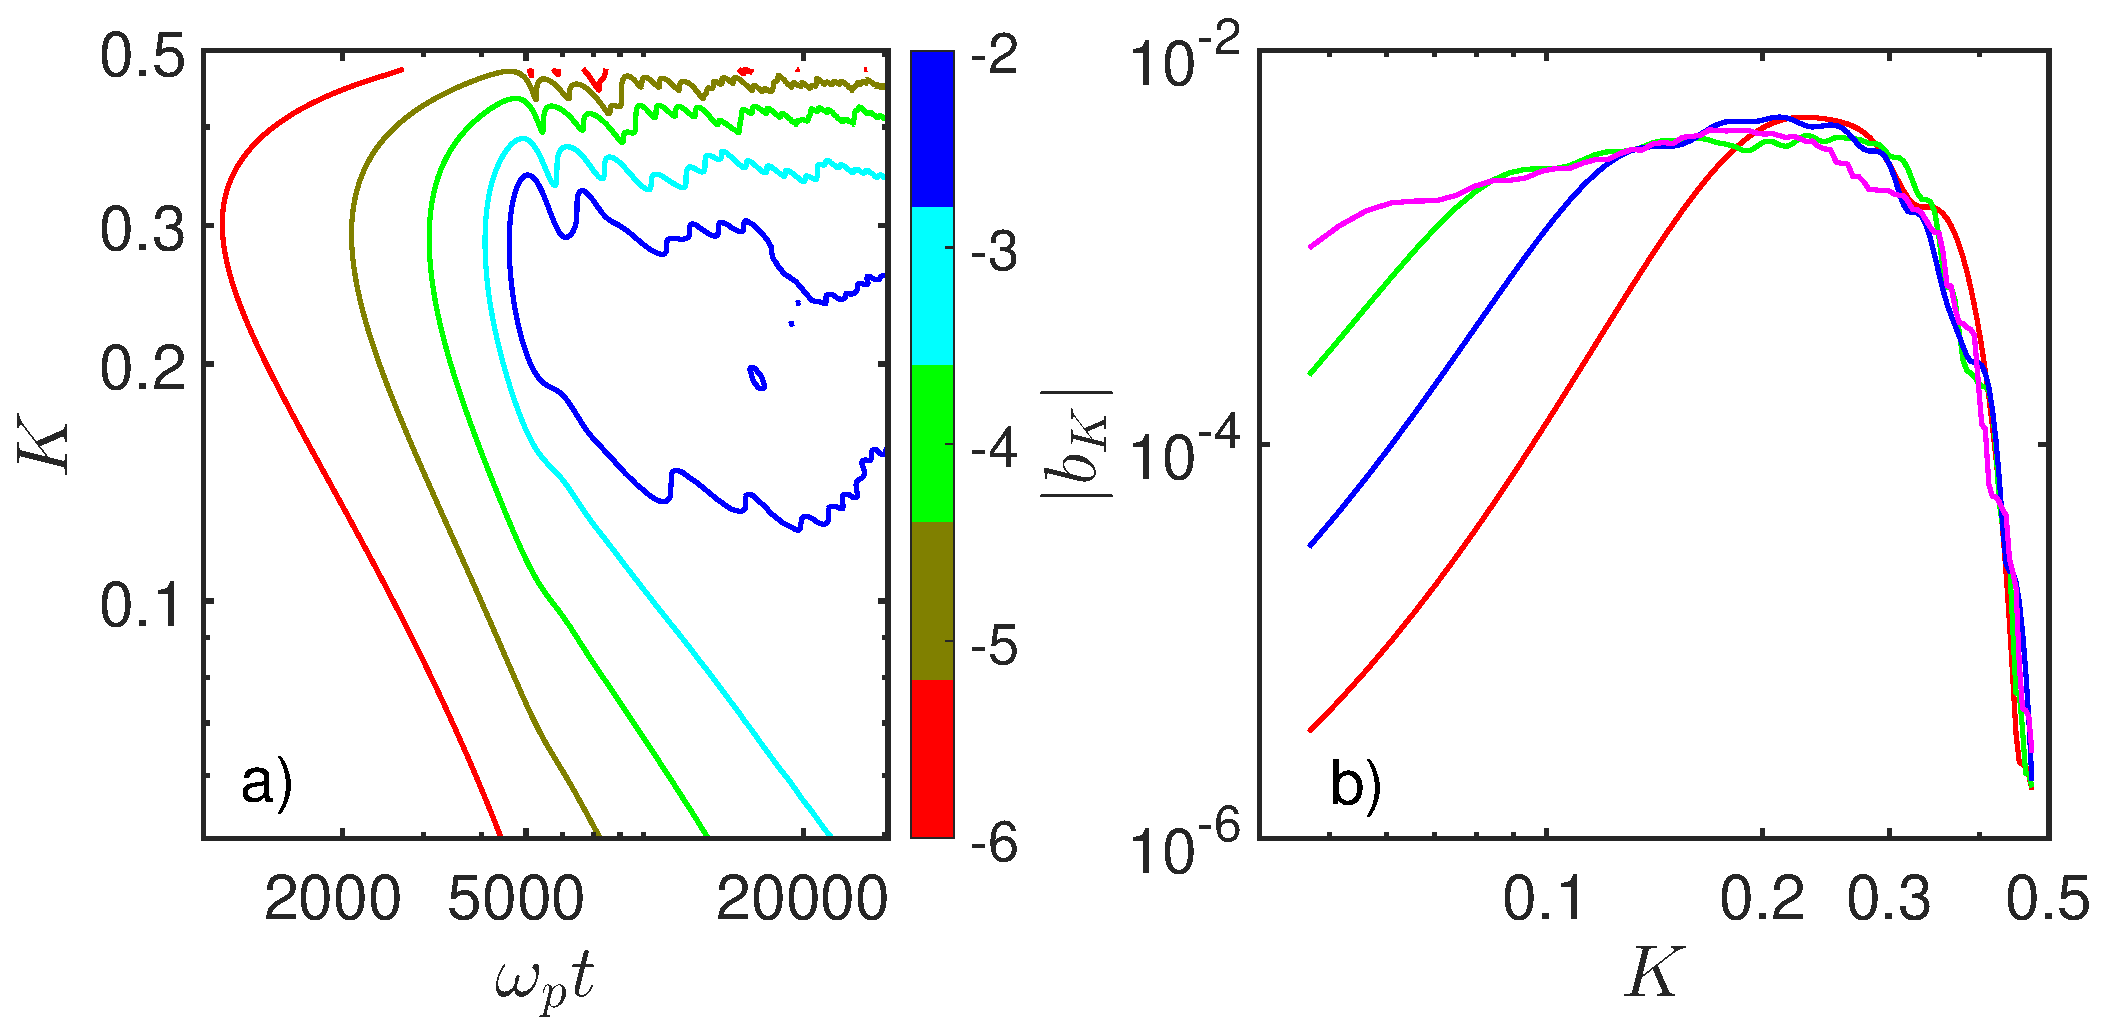
\includegraphics[width=0.9\linewidth]{part1/fig6.eps}
\caption{Эволюция спектра турбулентности, найденная в 1-мерном квазилинейном расчете, в двойном логарифмическом масштабе: (a)~линии уровня логарифма амплитуд мод магнитного поля $|b_K|$; 
(b)~спектр $|b_K|$ магнитного поля в моменты времени $\wpl t$, равные 6000 (красный цвет), 10000 (синий), 16000 (зеленый), 24000 (розовый). Начальная анизотропия $A_0=0.25$.}
\label{fig:dinspectrA025_1d}
\end{figure}

\begin{figure}[h]
\centering
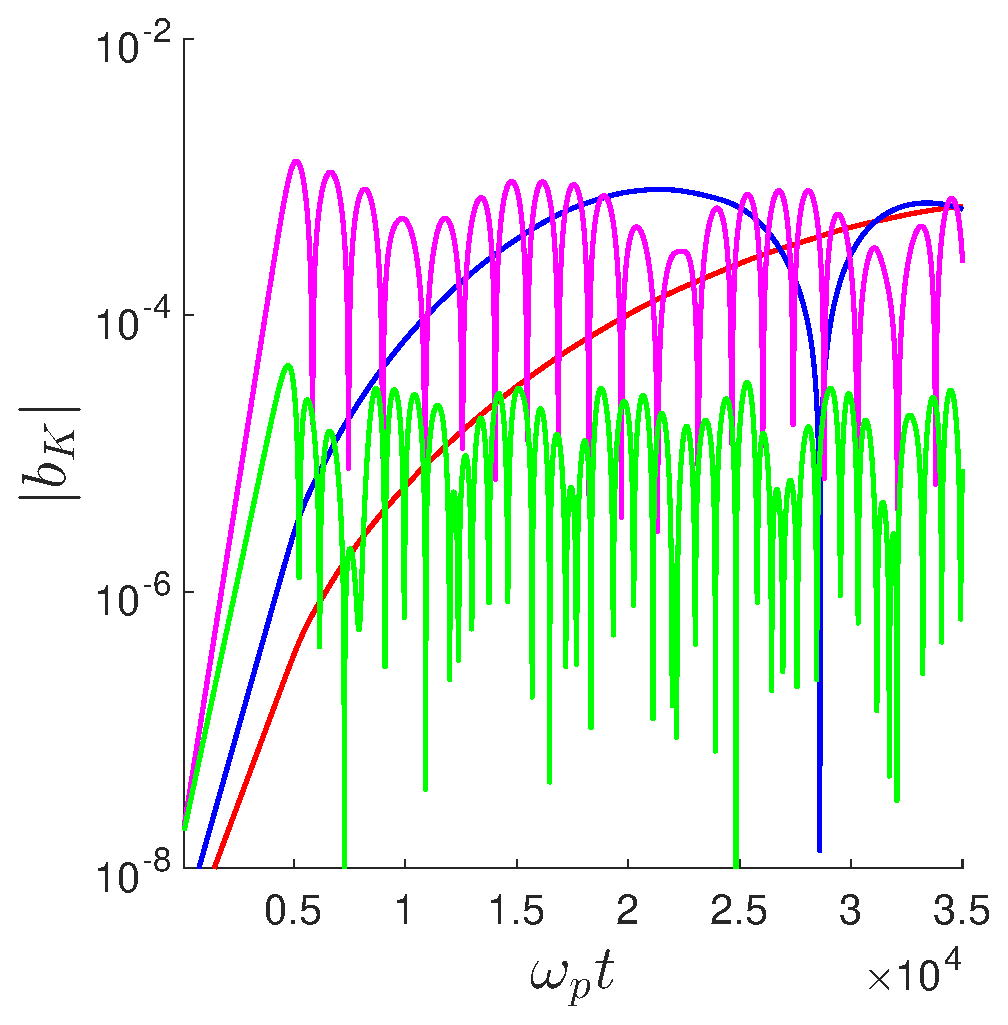
\includegraphics[width=0.65\linewidth]{part1/fig7.eps}
\caption{Эволюция четырех типичных мод ($K=0.08$ --- красный цвет, $K=0.11$ --- синий, $K=0.3$ --- розовый, $K=0.4$ --- зелёный), взятых из спектра рис. \ref{fig:dinspectrA025_1d}. Оптимальное волновое число $K_\mathrm{opt}\approx0.28$.}
\label{fig:evol_garmA025_1d}
\end{figure}

Типичные эволюция всего спектра и динамика отдельных мод на временах порядка десяти времен достижения насыщения наиболее неустойчивой моды с волновым числом $K_{opt}\approx0.28$ показаны на рис. \ref{fig:dinspectrA025_1d} и \ref{fig:evol_garmA025_1d}. 
Для определенности в квазилинейном моделировании в качестве начального использовался равномерный спектр мод с заданной малой амплитудой. 
Чем она ниже, тем сильнее в ходе первоначального экспоненциального роста спектр сужается около моды с волновым числом $K_{opt}$, приобретая колоколообразный вид функции Гаусса. 
Доминирующие моды с близкими волновыми числами, формирующиеся к моменту насыщения, вступают в квазилинейное взаимодействие и деформируют центральную часть функции распределения, ограничивая свой рост и рост коротковолновых мод, но позволяя расти более длинноволновым модам. 
Коротковолновое крыло спектра, которое лежит справа от моды с волновым числом $K_{max}$, обладающей наибольшей амплитудой магнитного поля, имеет довольно сложную форму, но в целом допускает крутую степенную аппроксимацию.

Значительная часть длинноволнового крыла спектра, которая примыкает к плато, образованному насытившими свой рост модами, на протяжении длительного промежутка нелинейной эволюции хорошо аппроксимируется степенной зависимостью с показателем, примерно равным 5 и мало меняющимся со временем; см. рис. \ref{fig:dinspectrA025_1d}b. 
Это обстоятельство дает основание для гипотезы о частичной автомодельности процесса. 
После насыщения неустойчивости среднее волновое число спектра $\langle K\rangle$ понемногу смещается в длинноволновую сторону. 
Одновременно с этим немного растет и дисперсия спектра $\sigma^2=\langle K^2\rangle-\langle K\rangle^2$ (см. (\ref{eq:angles})), которая снижалась на линейной стадии развития неустойчивости. 
Возможная связь указанной эволюции спектра с формированием или разрушением долгоживущих токовых слоев в одномерной вейбелевской турбулентности еще не изучалась.

На рис.~\ref{fig:evol_garmA025_1d} представлена характерная эволюция амплитуд мод с учетом их квазипериодических осцилляций (которые замываются при сложении мод и не видны при визуализации спектра на рис. \ref{fig:dinspectrA025_1d}, где проведено усреднение по близким модам). 
Пока мода с наибольшим инкрементом не достигнет насыщения, остальные моды растут экспоненциально со своими (разными) инкрементами и не испытывают осцилляций. 
После этого момента времени моды вблизи оптимальной и более коротковолновые моды тоже практически сразу насыщаются и начинают довольно быстро колебаться, почти не меняя своей амплитуды, т.е. у них величина инкремента значительно ниже появившейся действительной частоты. 
Вместе с тем более длинноволновые моды с инкрементом значительно меньше максимального продолжают нарастать, правда, почти по степенному закону с различными показателями порядка 3--5, достигают амплитуды порядка максимальной амплитуды моды с оптимальным волновым числом $K_{opt}\approx0.28$ и только после этого начинают медленно осциллировать с почти не уменьшающимся уровнем огибающей. 
Такая динамика мод согласована с указанной выше эволюцией их полного спектра, имеющей автомодельные черты.

Согласно даваемой аналитической теорией~\cite{Pokhotelov2011} оценке уровня насыщения эволюционного параметра $h$ в зависимости от начального параметра анизотропии, нетрудно оценить средний квадрат нормированного насыщающего магнитного поля (см.~(\ref{eq19plus1})), если учесть, что в момент насыщения неустойчивости в спектре доминируют моды с волновыми числами вблизи оптимального $K_\mathrm{opt}$, отвечающего наибольшему линейному инкременту:
\begin{equation}
\label{eq:analit_estimation}
b_{sat}^2\approx0.3\dfrac{A_0^5}{(1+A_0)^6} .
\end{equation}

Полученная оценка соответствует значениям насыщающего магнитного поля, найденным в одномерной задаче в рамках осуществленных квазилинейных расчетов, и дает его резкое спадание по закону $\approx 0.3 A_0^5$ при уменьшении начального параметра анизотропии~(рис.~\ref{fig:bsat}a). 
Для начальных параметров анизотропии больше единицы данная аналитическая оценка не применима, а численное моделирование показывает, что средний квадрат нормированного насыщающего поля с ростом параметра анизотропии стремится к величине чуть меньшей $0.1$~(рис. \ref{fig:bsat}b). 
При этом, как будет ясно из следующего подраздела, эволюция спектра одномерной турбулентности существенно изменяется. 
Кроме того, следует заметить, что в более реальном случае двумерной турбулентности, согласно рис. \ref{fig:bsat}b и главе \ref{ch:ch5}, не только меняется характер спектральной эволюции турбулентности, но и сама зависимость насыщающего магнитного поля от начального параметра анизотропии оказывается существенно другой, сильно отличающейся от~(\ref{eq:analit_estimation}) в сторону увеличения при малых $A_0$ и по-другому выходящей к максимальному значению при больших $A_0$; см., например,~\cite{Borodachev2010,Kuznetsov2022}. 

\begin{figure}[h]
\centering
\includegraphics[width=0.9\linewidth]{part1/fig8.eps}
\caption{Сравнение зависимостей среднего квадрата нормированного насыщающего магнитного поля $b_{sat}^2$ от начального параметра анизотропии $A_0$ (a) согласно оценке~(\ref{eq:analit_estimation}) (черный цвет) и численному квазилинейному моделированию по уравнениям (\ref{eq:f0.3})--(\ref{eq:max_eq}) (красный цвет); (b) согласно этому же моделированию (красный цвет) и расчетам методом частиц в ячейках с помощью кода EPOCH (синий цвет) в одномерном (штрихи) и двумерном (сплошная) случаях.}
\label{fig:bsat}
\end{figure}


\section{Эволюция одномерной вейбелевской турбулентности в случае высокой начальной анизотропии}\label{sec:ch1/sec4}

Если начальная анизотропия велика, $A_0\gg 1$, то исходные инкременты мод тоже велики, турбулентность развивается быстро и сразу в более широком интервале волновых чисел (вблизи оптимальной величины $K_\mathrm{opt}$ и существенно левее нее). 
На стадии насыщения роста этих мод функция распределения частиц значительно деформируется (в два и более раз) во всей области скоростей порядка тепловых, а не только вблизи своего максимума, как при $A_0\ll 1$. 
\begin{figure}[h]
\centering
\includegraphics[width=0.85\linewidth]{part1/fig9.eps}
\caption{(a)~Линии уровня $0.05$ (черный цвет), $0.1$ (красный), $0.5$ (зелёный) и $0.8$ (синий), отсчитанные от максимального значения функции распределения в момент времени $\wpl t =80$; (b)~то же в момент времени $\wpl t =440$; (c)~распределение частиц по величине нормированной компоненты скорости $\beta_x$, ортогональной оси анизотропии, в моменты времени $\wpl t$, равные 0 (красный цвет), 80 (черный) и 440 (зеленый). Приведены данные 1-мерного квазилинейного расчета при $A_0=10$.}
\label{fig:sravnenie_FR1d_A10}
\end{figure}

\begin{figure}[h]
\centering
\includegraphics[width=0.8\linewidth]{part1/fig10.eps}
\caption{Эволюция (a) среднеквадратичного магнитного поля $b_{av}$ (сплошная линия) и оценки этой величины~(\ref{eq:otsenka})~(штрихи), а также (b) параметра анизотропии $A$ согласно численному квазилинейному моделированию (красный цвет) и расчетам методом частиц в ячейках (синий цвет) в 1-мерной задаче при $A_0=10$.}
\label{fig:evol1d_QL_A10}
\end{figure}

Согласно расчетам, проведенным для определенности при $A_0=10$ (см. рис. \ref{fig:sravnenie_FR1d_A10} и ср. рис.~\ref{fig:sravnenie_FR1d}), в данном процессе происходит быстрое увеличение поперечной к оси анизотропии скорости электронов, двигавшихся сначала преимущественно вдоль этой оси, так что центральная часть распределения в значительной мере переходит на периферию и его форма вместо овальной приобретает прямоугольный вид с характерным отношением сторон порядка текущего значения параметра анизотропии $A$ после этапа насыщения. 
Это значение в несколько раз меньше исходного $A_0$, в рассмотренном примере - приблизительно в 5 раз, и в дальнейшем почти не уменьшается ($A\approx 2$, см. рис. \ref{fig:evol1d_QL_A10}). 
Практически не меняется и форма функции распределения частиц, остающаяся сильно отличной от бимаксвелловской, а также среднеквадратичная величина магнитного поля турбулентности. 
(Небольшие различия в слабом изменении среднеквадратичного поля $b_{av}$ после достижения им максимума, обнаруживаемые, с одной стороны, квазилинейным расчетом и, с другой стороны, при помощи кода EPOCH, обусловлены, по-видимому, неучтенными нелинейными эффектами в первом и численными шумами, искажающими и тормозящими эволюцию спектра, во втором.) 

Сравнивая эволюцию спектров турбулентности при высокой (рис.~\ref{fig:dinspectrA10_1d}) и низкой (рис.~\ref{fig:dinspectrA025_1d}) начальной анизотропии, заметим, что в первом случае затухание насытившихся, более коротковолновых мод оказывается значительно сильнее и автомодельный характер эволюции обоих крыльев спектра выражен более явно, чем во втором. 
Поэтому в случае высокой начальной анизотропии дисперсия спектра $\sigma^2=\langle K^2\rangle-\langle K\rangle^2$ заметно изменялась (уменьшалась) только на стадии экспоненциального роста мод, а после кратковременного уширения с началом нелинейной стадии уменьшается очень слабо, стремясь к постоянному значению, в отличие от случая низкой начальной анизотропии, когда эта дисперсия после первоначального уменьшения на линейной стадии медленно увеличивается за счет нелинейного (квазилинейного) роста длинноволнового крыла спектра. 
При этом среднее волновое число спектра $\langle K\rangle$ в первом случае со временем уменьшается примерно по степенному закону $t^{-1/2}$, тогда как во втором оно уменьшается весьма незначительно. 
Наконец, в первом случае, при $A_0=10$, близкий к степенному вид обоих крыльев спектра $|b_{k}|$ прослеживается гораздо более четко и практически сразу после насыщения роста среднеквадратичного поля, характеризуясь почти не меняющимися показателями около 10 и -13 в длинноволновой и коротковолновой частях соответственно, хотя эти показатели весьма чувствительны к начальному уровню амплитуд мод. 
Заметим, что во втором случае, при $A_0=0.25$, степенной вид принимает только длинноволновое крыло, причем с показателем примерно вдвое меньшем, т.е. около 5, и тоже чувствительным к начальному уровню амплитуд мод.

\begin{figure}[h]
\centering
\includegraphics[width=0.8\linewidth]{part1/fig11.eps}
\caption{Эволюция спектра турбулентности, найденная в 1-мерном квазилинейном расчете, в двойном логарифмическом масштабе: (a)~линии уровня логарифма амплитуд мод магнитного поля $|b_K|$; (b)~спектр $|b_K|$ магнитного поля в моменты времени $\wpl t$, равные 60 (красный цвет), 100 (синий), 180 (зеленый) и 360 (розовый). Начальная анизотропия $A_0=10$.}
\label{fig:dinspectrA10_1d}
\end{figure}

\begin{figure}[h]
\centering
\includegraphics[width=0.5\linewidth]{part1/fig12.eps}
\caption{Эволюция четырех типичных мод ($K=0.4$ --- красный цвет, $K=0.7$ --- синий, $K=1.2$ --- розовый, $K=1.6$ --- зелёный), взятых из спектра рис. \ref{fig:dinspectrA10_1d}. Оптимальное волновое число $K_\mathrm{opt}\approx1.2$.}
\label{fig:evol_garmA010_1d}
\end{figure}

Для сформировавшейся сложно анизотропной функции распределения большинство мод приобретают действительную частоту больше или порядка величины инкремента (декремента), а следовательно, их амплитуды $|b_{k}|$ начинают осциллировать, что отмечалось в предыдущем подразделе при $A_0=0.25$. 
Теперь, при $A_0=10$, это показано на рис.~\ref{fig:evol_garmA010_1d}, где частота осцилляций выше у более коротковолновых мод, причем для менее коротковолновых мод имеется промежуточная стадия примерно степенного роста (с различными показателями степени, опять, порядка 3-5, как и при $A_0=0.25$), начинающаяся почти сразу после момента насыщения моды с наибольшим исходным инкрементом и оптимальным волновым числом $K_\mathrm{opt}\approx1.2$ и заканчивающаяся моментом их собственного насыщения, после которого и возникают указанные осцилляции их амплитуд. 
Дальнейшее затухание огибающих этих осциллирующих амплитуд теперь выражено весьма сильно и является примерно экспоненциальным, а не степенным. 
Оно идет с разными декрементами в диапазоне 0.01-0.05 для различных мод, опускающихся вплоть до уровня численных шумов порядка $10^{-5}$. 
Осцилляции не наблюдаются только для наиболее длинноволновых мод, дисперсия которых, по-видимому, определяется уплощенной частью функции распределения, а их действительные частоты могут быть даже меньше их инкрементов (декрементов).

Согласно проведенному сравнительному анализу расчетов в рамках квазилинейного подхода и расчетов методом частиц в ячейках для указанных и других значений параметра анизотропии $A_0$, подобная динамика отдельных мод и спектра в целом в одномерной задаче обусловлена в основном чисто квазилинейными эффектами благодаря продолжающей самосогласованно изменяться функции распределения частиц. 
Тем не менее, из-за наличия уже упоминавшихся значительных численных шумов в использованном коде EPOCH, искажающих форму функции распределения и квазилинейную динамику мод, открытым остается вопрос о количественной оценке возможной, пусть малой, роли четырехволнового взаимодействия в нарастании все более длинноволновых и затухании ранее возбудившихся коротковолновых мод, а следовательно, в формировании и поддержании степенной формы крыльев спектра одномерной вейбелевской турбулентности, особенно на поздних этапах ее затухания.




\section{Заключение} 

В данной главе описан и обоснован квазилинейный численный подход к описанию эволюции вейбелевской ТЕМ-турбулентности и соответствующей деформации функции распределения частиц, использующий приближение слабой нелинейной турбулентности, т.е. слабого взаимодействия ее пространственных мод (гармоник). 
Этот подход и развитые с его помощью представления о квазимагнитостатической турбулентности являются универсальными, т.е. применимы к различным исходным функциям распределения частиц по скоростям, включая не только бимаксвелловские, но и бикаппа-, комбинированные пучковые, не осесимметричные и другие распределения, представляющие интерес в различных ситуациях в плазме, включая наличие внешнего магнитного поля. 
В одномерной задаче полученные решения квазилинейных уравнений качественно согласуются с результатами имеющейся аналитической теории в пределах её применимости и позволяют анализировать недоступную ей динамику спектра турбулентности, в том числе в сильно анизотропной плазме. 

В итоге, общий сценарий эволюции спектра вейбелевской турбулентности, который по существу можно назвать квазилинейным, в рассмотренном одномерном случае представляется следующим. 
При небольшом уровне начальных шумов на линейной стадии неустойчивости анизотропной плазмы происходит экспоненциальный, апериодический рост мод в довольно широком интервале волновых чисел, для которых инкремент не сильно меньше максимального. 
К моменту насыщения роста среднеквадратичного магнитного поля профиль спектра может значительно сузиться и центральная группа его мод, следуя квазилинейной динамике и за счет <<квадратичной>> нелинейности возбуждая вторые гармоники функции распределения частиц и деформируя среднюю по пространству форму этой функции, начинает существенно уменьшать средний параметр анизотропии и инкремент всех мод, причем для указанных центральных мод последний становится даже отрицательным. 
В результате коротковолновое крыло спектра постепенно затухает, а длинноволновое продолжает расти, причем там темп роста амплитуд мод почти сразу после момента насыщения становится примерно степенным (вместо экспоненциального или нелинейно индуцированного) с показателем, зависящим от волнового числа моды: более длинноволновые моды нарастают медленнее менее длинноволновых. 
В ходе процесса максимальными амплитудами по очереди начинают обладать все более длинноволновые моды, и величина этого максимума сначала даже немного растет (в области пологого плато на зависимости среднеквадратичного магнитного поля от времени), а потом начинает медленно убывать

Необходимо подчеркнуть, что представленная плавная в целом динамика спектра как большого случайного набора изначально апериодических вейбелевских мод складывается из колебательного поведения почти всех мод, наступающего практически сразу после насыщения роста энергии турбулентности, когда функция распределения частиц по скоростям не только выполаживается, но и приобретает сложную небимаксвелловскую форму, постепенно меняющуюся со временем. 
Следуя изменившейся дисперсии плазмы, моды приобретают различные действительные частоты, вообще говоря, сравнимые с их изменившимися инкрементами (или декрементами), и начинают по-разному осциллировать, продолжая нарастать (или затухать). 
Развитый квазилинейный подход хотя и не содержит в явном виде решение дисперсионного уравнения, но в полной мере учитывает данное важное обстоятельство, обычно скрытое численными шумами при моделировании методом частиц в ячейках. 


Ограничение квазилинейного подхода и обуславливающие его неучтенные нелинейные эффекты могут проявляться кратковременно или накапливаться в ходе долговременной эволюции спектра мод, причем результат зависит от характера анизотропии плазмы и геометрии задачи. 
В главе \ref{ch:ch2} будет продемонстрировано, что двумерной аксиальносимметричной задаче на продолжительном промежутке эволюции, многократно превосходящем время до насыщения неустойчивости, квазилинейный подход корректно описывает спектральную динамику незамагниченной турбулентности за исключением кратковременного обогащения коротковолнового крыла спектра за счет генерации суммарных гармоник сразу после начала насыщения турбулентности (см. также~\cite{Garasev2021}). 
В главе \ref{ch:ch4} будет показано, что при наличии достаточно сильного внешнего магнитного поля, даже ориентированного вдоль оси анизотропии и не нарушающего аксиальную симметрию задачи, такие эффекты могут дополнительно расширять спектр мод на этапе насыщения не только в коротковолновой, но и в длинноволновой области.  
В следствие этого, основная энергонесущая часть спектра смещается в длинноволновую область за счет нелинейного взаимодействия, не учитываемого в квазилинейном подходе.
